
\subsection*{Introduction}

Fused filament fabrication is a popular 3D fabrication process whereby the molten materials are deposited layer by layer. Supporting structures are fabricated concurrently and act as a fixture to support the weights of material that constitute the overhanging regions. Supporting structures introduce material waste and prolong the time required for fabrication. Additionally, they often require manual removal and could potentially introduce damage to the model itself. It is desirable to print models with minimal supporting structures.

There are several approaches to the problem.~\cite{jiang_xu_stringer_2018} One approach focuses on finding the best printing orientation and designing better support generation algorithms.~\cite{vanek_galicia_benes_2014} Alternatively, people have incorporated support structure constraints to topology optimization during model design.~\cite{langelaar_2016} The most relevant approach to this abstract relies on deforming the shape itself for self-support in situation where the geometry of the shape is not critical. There has been attempt to reduce the number of overhanging regions iteratively by deforming an enclosing coarser volumetric mesh.~\cite{hu_jin_wang_2015}.

Linear blend skinning is a fast deformation method. Recent work shown impressive result in automatically generating weights for smooth and intuitive deformation~\cite{jacobson_bounded_biharmonic_weights_2011} and in efficiently computing as-rigid-as-possible deformations by searching in the subspace of skinning deformations.~\cite{jacobson_fast_2012}.

This abstract presents a method for finding natural deformations with reduced support structures. We pose the problem of support reduction as a global optimization problem over the space of linear blend skinning deformations minimizing several objectives, namely
\begin{enumerate}
    \item local distortion ~\cite{sorkine_arap_2007}
    \item support structures
    \item self-intersection
\end{enumerate}
We implemented a prototype and fabricated some model for visualization.

\subsection*{Method}

Let $\calM = (\bV, \bF)$ be rest-pose mesh living in dimension $d\in\{2,3\}$. Let $\bV = \{\bv_1^T, \cdots, \bv_n^T\}^T \in \R^{n \times d}$ be the rest-pose vertex positions. Let $\calM' = (\bV', \bF)$ be deformed mesh.

\subsubsection*{Linear Blend Skinning}

Given a set of handles $\calH = \{ \bh_1, \cdots, \bh_m \}$, we can apply an affine transformation $\bT_j \in \R^{d \times (d+1)}$ on each handle $\bh_j$. Let $\bT = \{ \bT_1^T, \cdots, \bT_m^T \}^T \in \R^{(d+1)m \times d}$. Linear blend skinning is a deformation method whereby the vertex positions on the deformed shape are represented as a weighted linear combination of the handles' transformations,
\[
    \bv_i' = \sum_{j=1}^m w_j(\bv_i) \bT_j 
    \begin{pmatrix} 
    \bv_i \\
    1 
    \end{pmatrix} 
\]
where $w_j: \calM \rightarrow \R$ is computed using bounded biharmonic weights.\cite{jacobson_bounded_biharmonic_weights_2011} Equivalently, $\bV' = \bM \bT$, where $\bM \in \R^{n \times (d+1)m}$ is a matrix combining $\bV$ and $\bW$ as noted in \cite{jacobson_fast_2012}. 

% Note that the energies below are a function of $\bV'$, and hence a function of $\bT$ if we substitute $\bM \bT$ in its place, i.e. 
% \[
%     E_{arap}(\bT) = E_{arap}(\bT, \bM) = E_{arap}(\bV')
% \]
% where $\bM$ is fixed.

% \subsubsection*{Energy Formulation}

% We formulate objectives as stated prevously as functions of deformed vertex positions. Let $E,E_{arap},E_{overhang},E_{intersect} : \R^{n\times d} \to \R$ where $E$ is a weighted sum of 3 energy functions
% \[
%     E = \omega_1 E_{arap} + \omega_2 E_{overhang} + \omega_3 E_{intersect}
% \]


\subsubsection*{As-rigid-as-possible Energy}

To obtain natural deformations, we minimize a distortion energy $E_{arap}:  \R^{n \times d} \to \R$ which measures local deviation from rigidity and acts to preserve shape detail.~\cite{sorkine_arap_2007}
\[
    E_{arap}(\bV') = \frac{1}{2} \sum_{f\in \bF} \sum_{(i,j)\in f} c_{ijf} || (\bv_i' - \bv_j') - \bR_f(\bv_i - \bv_j) ||^2
\]
where $\R_f \in SO(d)$ are per-face rotations and $c_{ijk}\in \R$ are cotangent weights. Let $\R = \{\R_1^T, \cdots, \R_f^T, \cdots, \R_n^T \}^T \in \R^{dn \times d}$. We can find $\bR$ in local step before computing $E_{arap}$,
\[
    \bR = \argmin_{\bR} tr(\bR\tilde{\bK}\bT)
\]
as specified in \cite{jacobson_fast_2012} vis singular value decomposition.

% We can define the \textit{as-rigid-as-possible} deformation energy, which measures local distortion, to be
% \[
%     E_{arap}(\bV', \bR) = \frac{1}{2} \sum_{f\in \bF} \sum_{(i,j)\in f} c_{ij} || (\bv_i' - \bv_j') - \bR(\bv_i - \bv_j) ||^2
% \]
% Reformulating the ARAP energy to be a function of $\bV'$ only, we get
% \[
%     E_{arap}(\bV')
%     \qquad
%     \bR = \argmin_{\bR} tr(\bR\tilde{\bK}\bT)
% \]
% In matrix form, this becomes
% \begin{align*}
% E_{arap}(\bV') 
%     &= tr(\frac{1}{2}\bV'^T \bL \bV' + \bV'^T \bK \bR ) \\
%     &= tr(\frac{1}{2}\bT^T \tilde{\bL} \bT + \bT^T \tilde{\bK} \bR)
% \end{align*}
    
% where $\tilde{\bL} = \bM^T \bL \bM \in \R^{(d+1)m \times (d+1)m}$, $\tilde{\bK} = \bM^T \bK \in \R^{(d+1)m \times dn}$ and $\bK$ as defined in the deformation assignment

\subsubsection*{Overhang Energy}

An overhanging region that can be 3D printed without support is called \textit{self-supported}. We call the angle between the region's tangent plane and printing direction the \textit{self-supported angle} $\alpha$. Let $\alpha_{max}$ be the maximum supporting angle. Let $\tau = \sin(\alpha_{max})$ be the \textit{maximal supporting coefficient}. A surface $f\in \bF$ is considered \textit{risky} and thus requires support if,
\[
    \arccos(\bn_f \cdot \bd_{p}) > \pi + \alpha_{max}
    \quad \rightarrow \quad
    \bn_f \cdot \bd_{p} < - \tau
\]
where $\bn_f$ is unit normal of face $f$ and $\bd_{p}$ is the printing direction. Let $\partial \calM' \subset \bF$ be surface faces of the deformed mesh. Let $A(\cdot)$ be the area function and $c(\cdot)$ be the centroid function for a face $f$. We can approximate the volume of support required for any face risky $f$ by computing the volume of a rectangular prism,
\[
    \lambda(f) = 
    \begin{cases}
        A_{base} h = A_f |\bn_f \cdot \bd_{p}| (\bc_f \cdot \bd_{p}) & \text{if } \bn_f \cdot \bd_{p} < -\tau \\
        0 & otherwise \\
    \end{cases}
\]
where $A_f$ is the area of the face, $\bc_f$ is the centroid of the face. We define an overhang energy $E_{overhang}: \R^{n\times d} \to \R$ which measures the volume of support required,
\[
    E_{overhang}(\bV') = \sum_{f\in \partial \calM'} \lambda(f)
\]

\subsubsection*{Self-intersection Energy}

One dominant artifact in skinning deformation is self-intersection, which renders the shape not 3D printable. We call a subset of mesh $\calM$ bordered by intersecting tetrahedra the \textit{self-intersecting region}. To quantify the total volume $V_i$ of each self-intersecting region, we define a $k\times k$ grid below the mesh and trace rays up in direction of the printing direction from every grid point. A ray is inside a self-intersecting region if $\bd_{p} \cdot \bn_f < 0$ for 2 consecutively incident faces. Summation of distances $d_j$ that $j$-th ray traversed inside a self-intersecting region approximates the volume. We can define a self-intersection energy $E_{intersect}: \R^{n\times d} \to \R$ which measures the total volume of the self-intersecting regions as follows,
\[
    E_{intersect}(\bV') = \sum_i V_i = \sum_{j=1}^{k\times k} d_j
\]

% traversed inside each region 




% To minimize self-intersection, we define a \textit{self-intersection energy}

% To prevent ARAP from deforming the mesh in such a way as to cause self-intersections, we add a third energy to measure them. We define a \textit{self-intersecting region} as the region inside the mesh that is bordered by intersecting tetrahedra. Given $j$ such regions we define the self-intersection energy to be
% \[
% 	E_{intersect}(\bV') = \sum_{i=1}^j V_i
% \]

% where $V_i$ is the volume of the $i^{\text{th}}$ region. To find these volumes, we define a grid below the mesh and trace a ray up from every grid point. If it enters the mesh twice in a row, we know the ray must be in a self-intersecting region. "Entering" simply means the direction of the ray is opposite to the vertical component of the normal direction of the surface at that point. When it exits this region, we record the distance the ray traversed inside it. The sum of all these lengths produces an approximation of the combined volume. The finer the grid, the more accurate the approximation.


\subsubsection*{Optimization}

We perform global optimization over the space of linear blend skinning transformations using particle swarm optimization, as noted in \cite{jacobson_matryoshka_2017}. We define a single objective function $E: \R^{3m} \to \R$ as a weighted sum of 3 energy functions,
\[
    E(\bx) = \omega_1 E_{arap}(\bV') + \omega_2 E_{overhang}(\bV') + \omega_3 E_{intersect}(\bV')
\]
where $\bx = \{ \phi_j, \theta_j, \psi_j \}_{j=1}^m$ are euler's angles describing the local rotation for each handle $h_j \in \calH$. We use forward kinematics to propagate local rotations $\bx$ in order to compute the transformation matrix $\bT$. We apply linear blend skinning formula $\bV' = \bM \bT$ to determine vertex positions for the deformed mesh, from which we can determine the value for as-rigid-as-possible, overhang, and self-intersection energy. $\omega_1,\omega_2,\omega_3$ are hyperparameters used to adjust relative weight of different objectives and are chosen a posteriori.

\subsection*{Experiments \& Results}

We use the same default settings for particle swarm optimization as specified in \cite{jacobson_matryoshka_2017} with 200 random initial particles and 120 iterations for both Figure.~\ref{fig:bb_bunny} and Figure.~\ref{fig:bunny}. By observing the viewer and fabricated model, we observe a reduction in the number of \textit{risky} faces as well as support materials used. The generated deformation are natural and has some but negligible self-intersection.

\begin{figure}[ht]
    \centering
    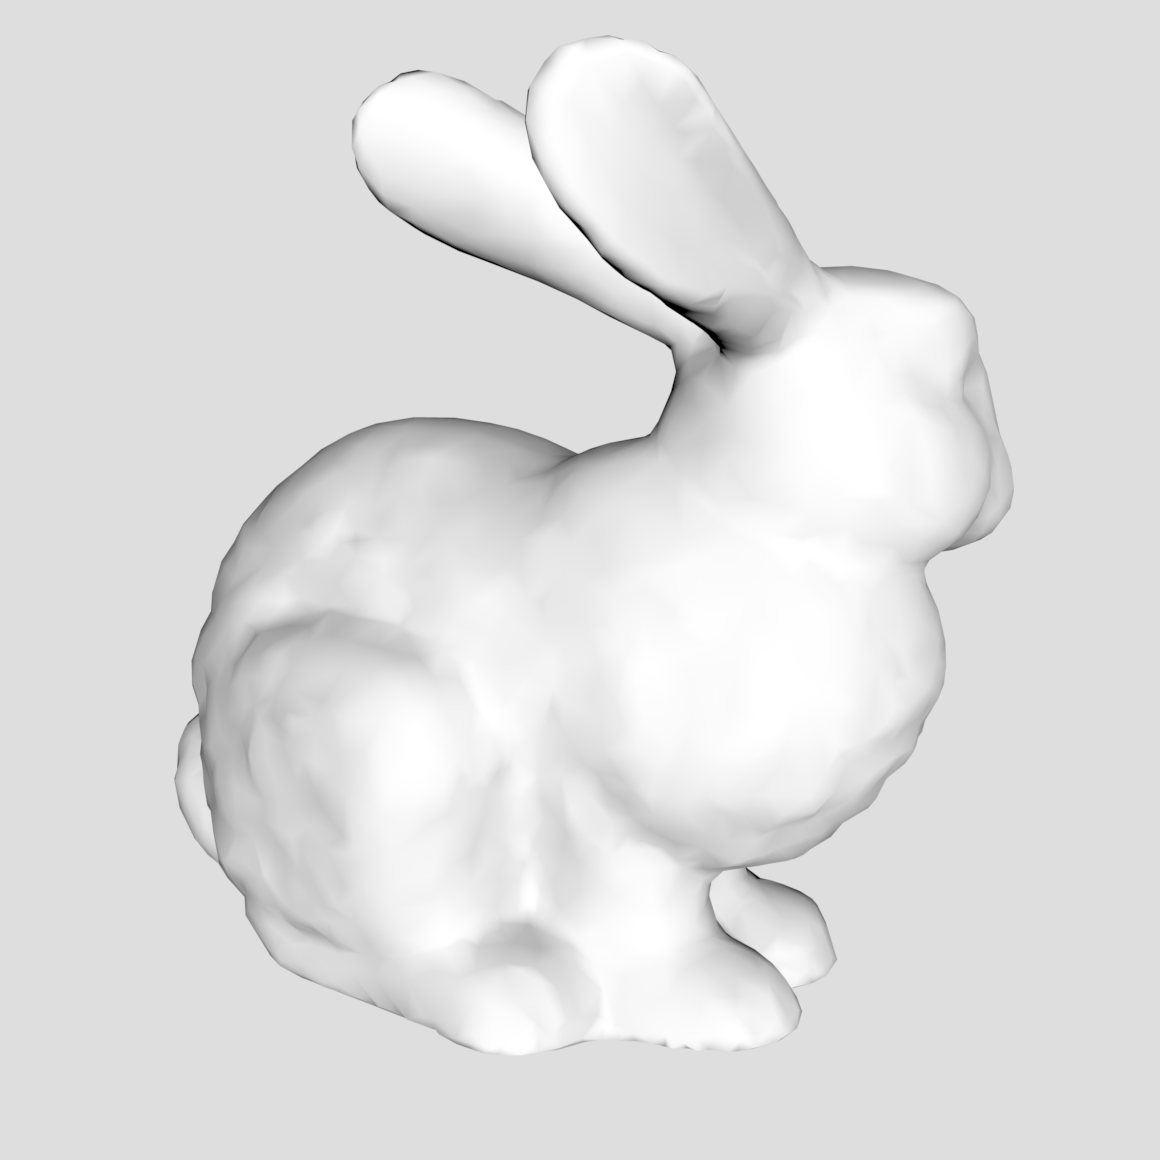
\includegraphics[width=0.13\textwidth]{bunny.png}
    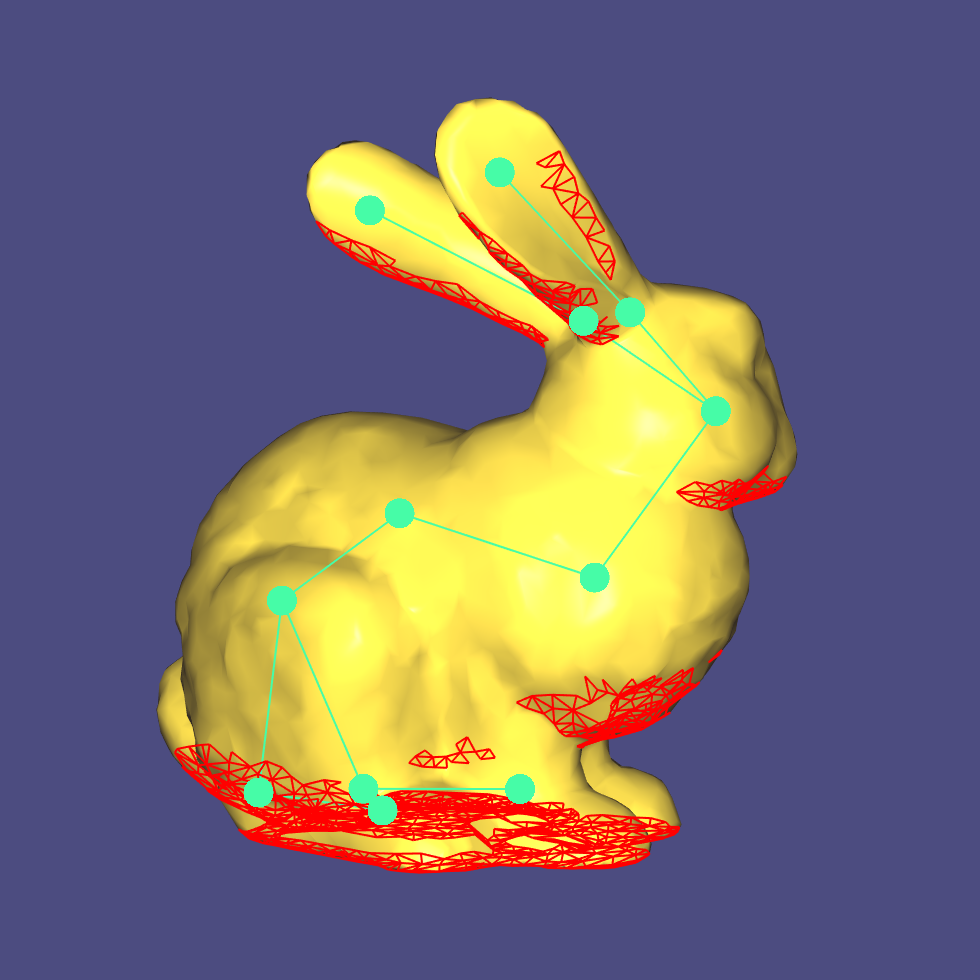
\includegraphics[width=0.13\textwidth]{bunny_igl.png} 
    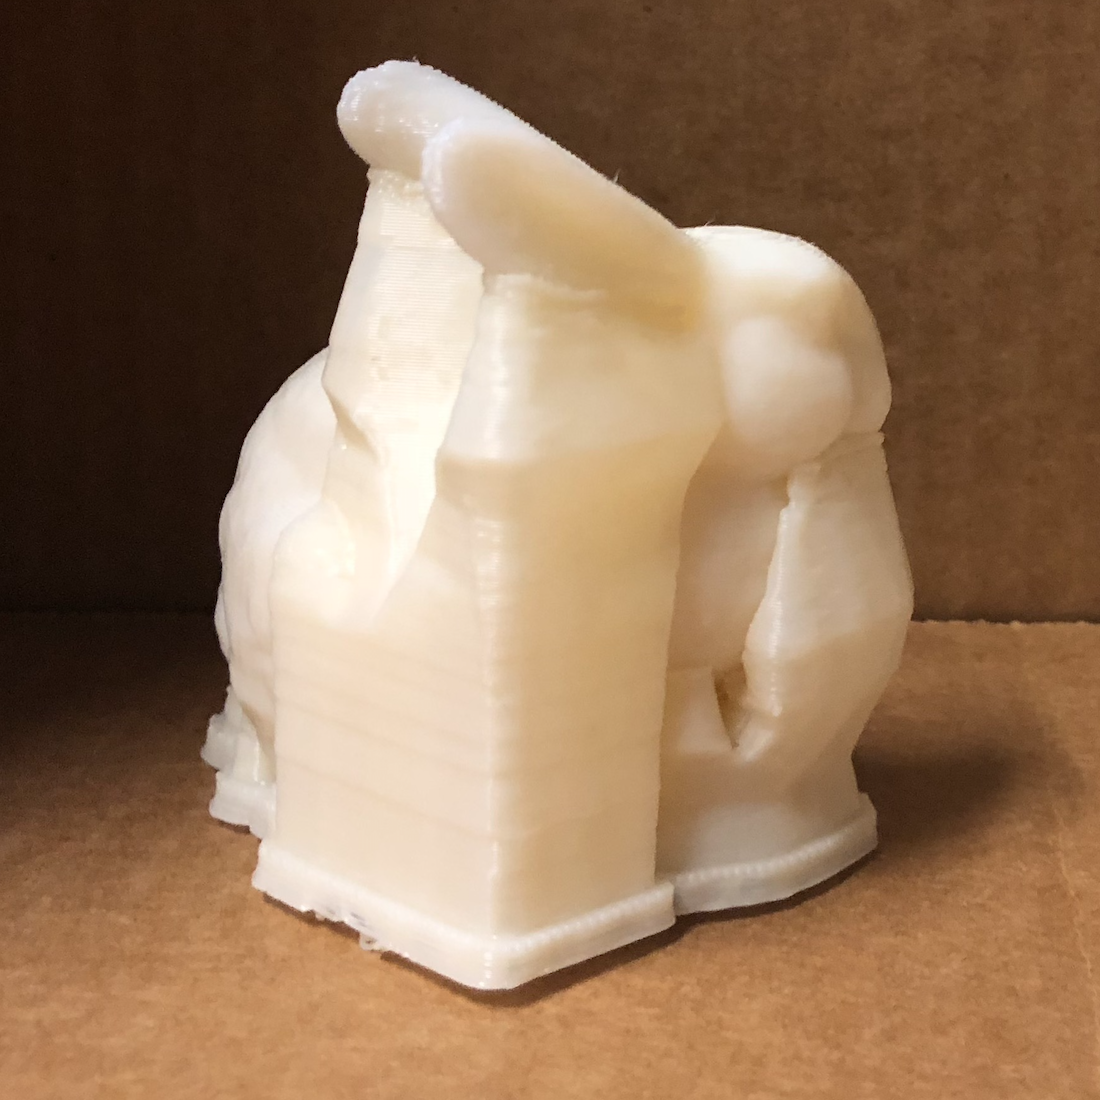
\includegraphics[width=0.13\textwidth]{bunny_3dp.png}
    \\
    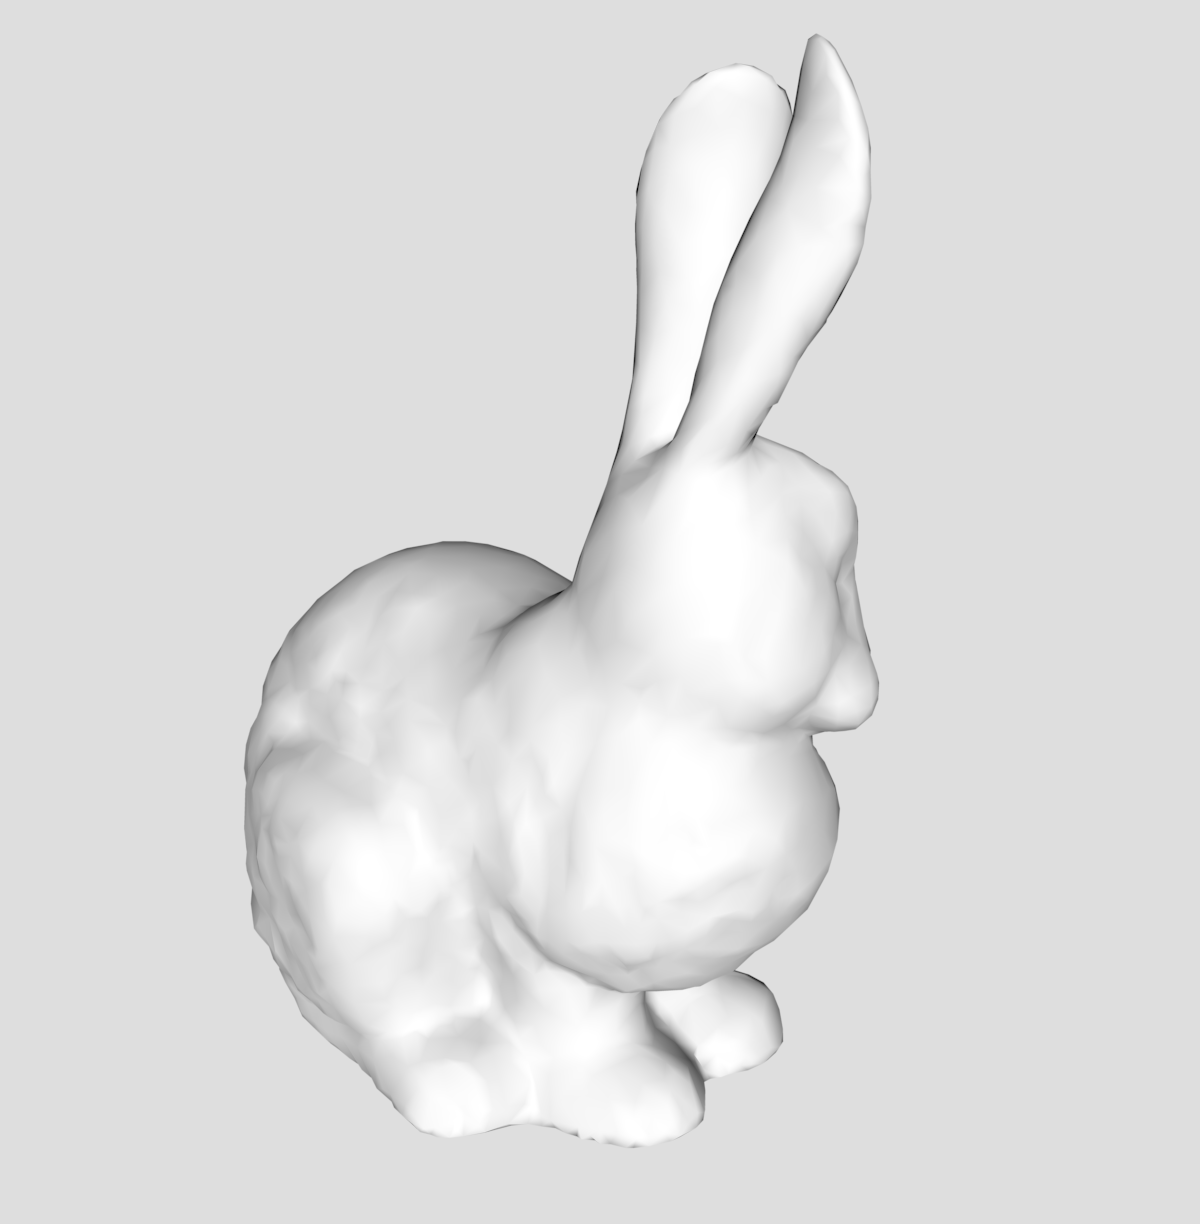
\includegraphics[width=0.13\textwidth]{bunny_deformed.png} 
    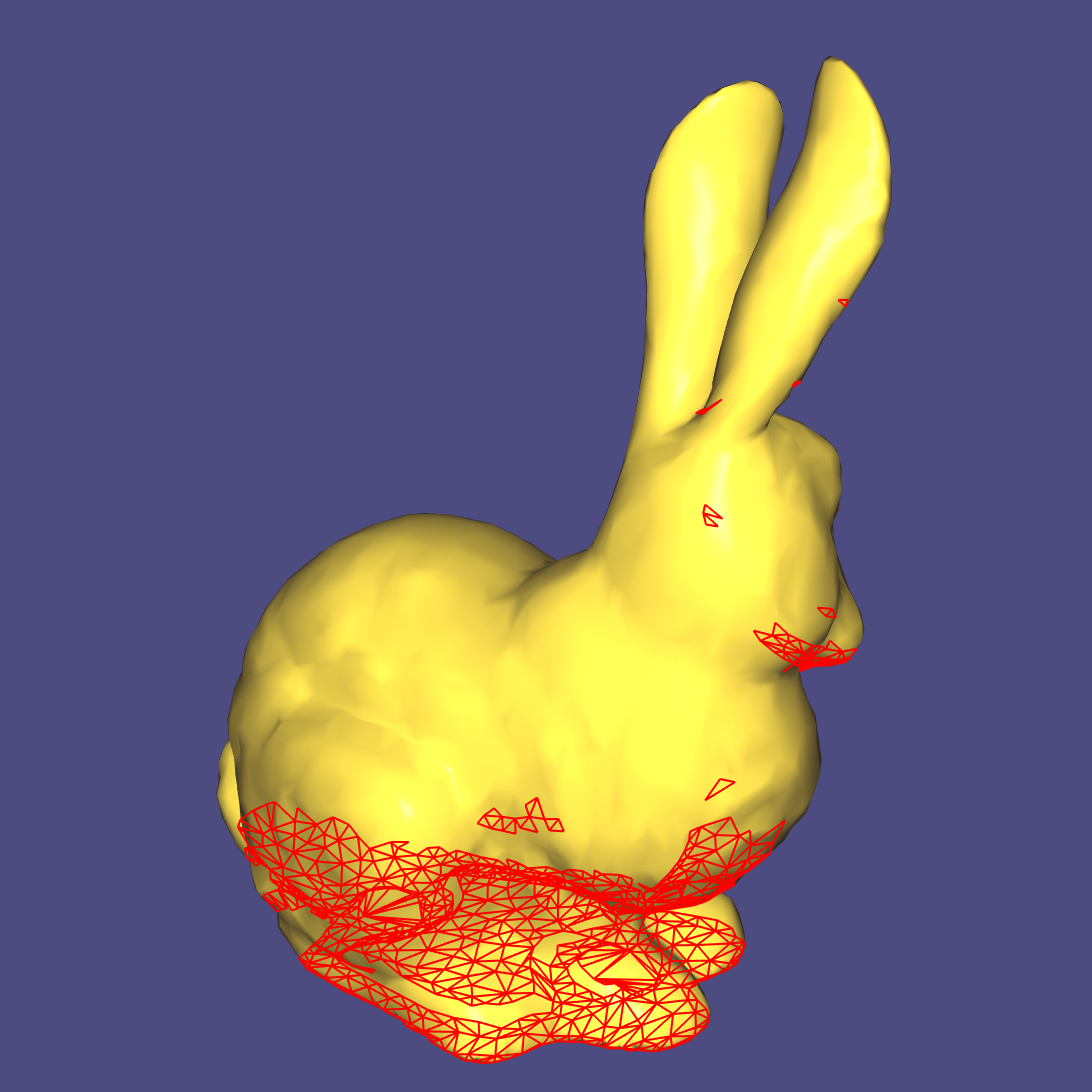
\includegraphics[width=0.13\textwidth]{bunny_deformed_igl.png} 
    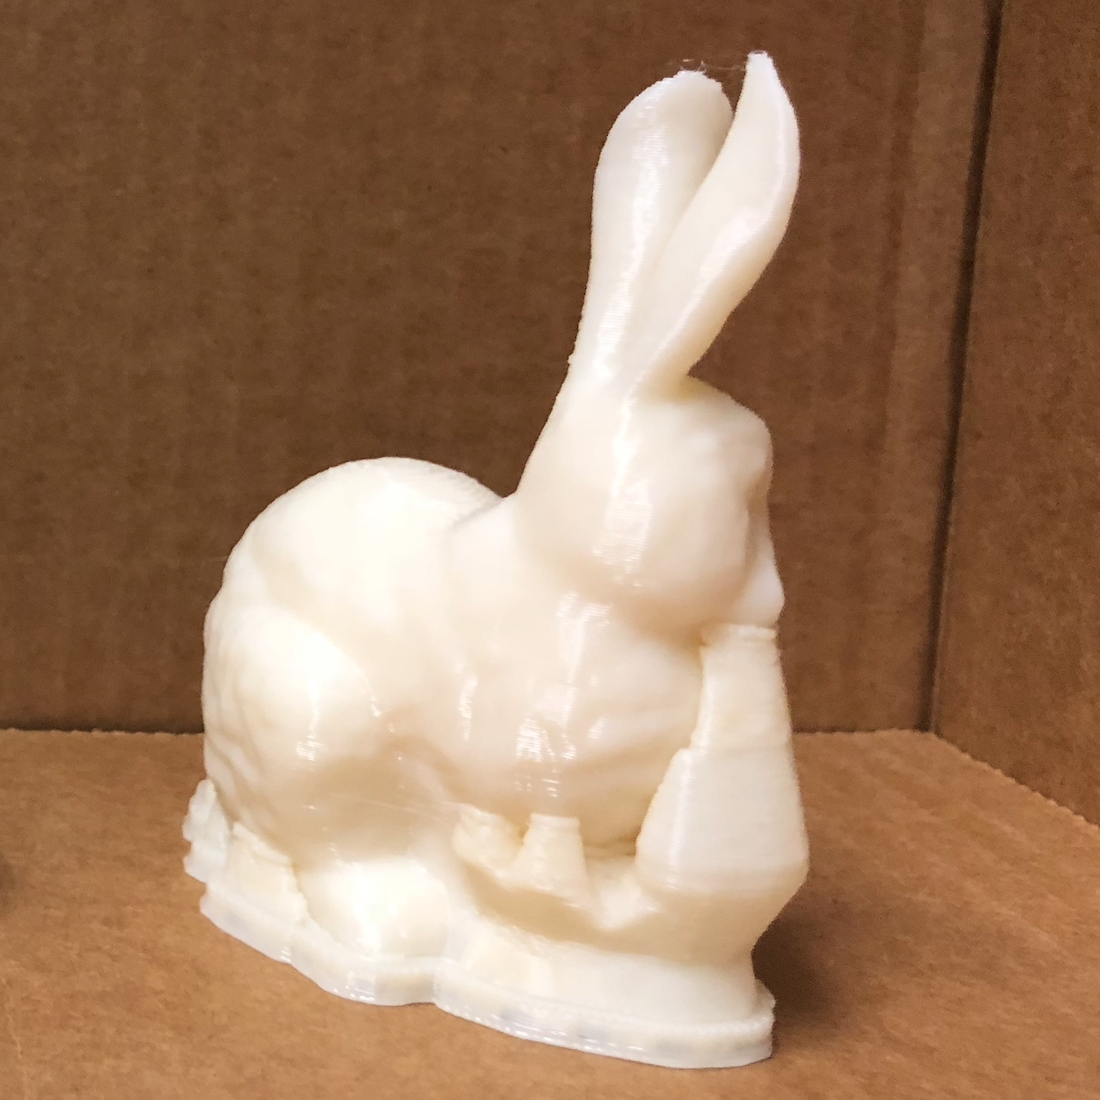
\includegraphics[width=0.13\textwidth]{bunny_deformed_3dp.png}
    \caption{Our method reduces support material usage by 37\% on the bunny}
    \label{fig:bunny}
\end{figure}


\subsection*{Limitations and Future Work}

Hyperparameters $\omega_1, \omega_2, \omega_3$ are tuned manually by experimentation and there is no clear way to pick sensible values because the objectives are tradeoffs and often act in conflict with each other. For example, overhang free deformation may introduce a large amount of distortions. In future work, we would like to investigate more on multi-objective optimization.

Currently, An entire run of the optimization procedure took several minutes for Figure.~\ref{fig:bb_bunny} and Figure.~\ref{fig:bunny}. There are huge potential in moving linear blend skinning and energy computation to vertex shaders for fast and parallel computation. In future work, we want to re-implement bottleneck steps using OpenGL for real time computation to allow for interactive design.

Although we have decided to look at support reduction, the method can be easily adapted to incoporate additional constraint. For example, we can formulate another energy term to account for center of mass for self-balancing.~\cite{make_it_stand_2013} or to account for the physical strength of the fabrication material. In future work, we want to include additional constraint to make 3D model self-support itself in a variety of scenarios.